\section{Đường tròn ngoại tiếp, nội tiếp tam giác} % Tên bài
\subsection{Đường tròn ngoại tiếp tam giác}
\subsubsection{Kiến thức trọng tâm}
\begin{tomtat}
	\immini{
		\begin{itemize}
			\item Đường tròn đi qua ba đỉnh của một tam giác gọi là \textit{đường tròn ngoại tiếp tam giác}, khi đó tam giác được gọi là \textit{tam giác nội tiếp đường tròn}.
			\item Đường tròn ngoại tiếp tam giác có tâm là giao điểm của ba đường trung trực của tam giác và có bán kính bằng khoảng cách từ giao điểm đó đến một đỉnh bất kì của tam giác.
		\end{itemize}
	}{
		\begin{tikzpicture}[>=stealth,line join=round,line cap=round,font=\footnotesize,scale=1]
			\def\r{2}
			\path 
			(0,0) coordinate (O)
			(100:\r) coordinate (A)
			(-40:\r) coordinate (C)
			(-140:\r) coordinate (B)
			($(A)!1/2!(B)$) coordinate (a)
			($(A)!1/2!(C)$) coordinate (b)
			($(C)!1/2!(B)$) coordinate (c)
			;
			\draw
			(O) circle (\r)
			(A)--(a)node[midway,sloped]{$|$}--(B)node[midway,sloped]{$|$}--(c)node[midway,sloped]{$||$}--(C)node[midway,sloped]{$||$}--(b) node[midway,sloped]{$|||$}--(A)node[midway,sloped]{$|||$}
			(A)--(O)
			(B)--(O)
			(C)--(O)
			pic[draw, angle radius=2mm]{right angle = O--a--A}
			pic[draw, angle radius=2mm]{right angle = O--b--A}
			pic[draw, angle radius=2mm]{right angle = O--c--B}
			;
			\draw[red] (O)--($(a)!1cm!180:(O)$)
			(O)--($(b)!1cm!180:(O)$)
			(O)--($(c)!1cm!180:(O)$)
			;
			\foreach \x/\g in {A/90,B/180,C/0,O/-5}
			\draw [fill=black](\x) circle (1pt) +(\g:3mm) node {$\x$};
		\end{tikzpicture}
	}
\end{tomtat}

\begin{vd}%[SGK CTST Toán 9]%[Dự án EX-9-Đề Cương Toán 9]%[Trần Thanh Phong]%[9H3N1-1]
	Cho hai đường tròn $(I)$ và $(J)$ cắt nhau tại $M$, $N$. Gọi $E$ và $F$ (khác $M$, $N$) là hai điểm lần lượt trên $(I)$ và $(J)$. Tìm đường tròn ngoại tiếp tam giác $MNE$ và đường tròn ngoại tiếp tam giác $MNF$.
	\begin{center}
		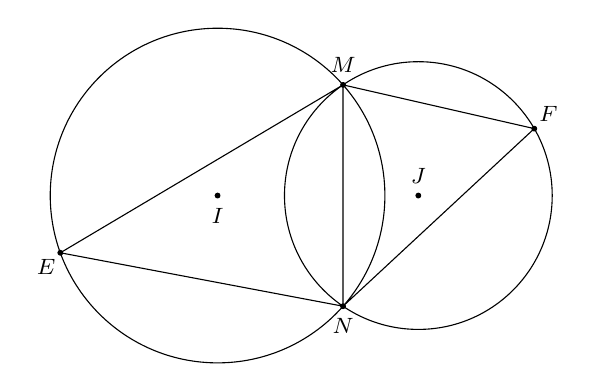
\begin{tikzpicture}[line join=round, line cap=round, >=stealth, font=\footnotesize, scale=0.85]
			\path
			(0,0) coordinate (I)
			(3,0) coordinate (J)
			(I) + ({atan2(sqrt(2.5*2.5 - ((2.5*2.5-2*2+3*3)/(2*3))*((2.5*2.5-2*2+3*3)/(2*3))), (2.5*2.5-2*2+3*3)/(2*3))}:2.5) coordinate (M)
			(I) + ({atan2(-sqrt(2.5*2.5 - ((2.5*2.5-2*2+3*3)/(2*3))*((2.5*2.5-2*2+3*3)/(2*3))), (2.5*2.5-2*2+3*3)/(2*3))}:2.5) coordinate (N)
			(I) + ({-160}:2.5) coordinate (E)
			(J) + ({30}:2) coordinate (F);
			
			\draw
			(I) circle (2.5)
			(J) circle (2)
			(M)--(N)
			(M)--(E)
			(N)--(E)
			(M)--(F)
			(N)--(F)
			;
			
			\foreach \point/\angle in {I/-90, J/90, M/90, N/-90, E/-135, F/45}
			\draw [fill=black] (\point) circle (1pt) +(\angle:3mm) node {$\point$};
		\end{tikzpicture}
	\end{center}
	\loigiai{
		Ta có đường tròn $(I)$ đi qua ba điểm $M$, $N$, $E$, suy ra $(I)$ là đường tròn ngoại tiếp tam giác $MNE$.\\
		Ta có đường tròn $(J)$ đi qua ba điểm $M$, $N$, $F$, suy ra $(J)$ là đường tròn ngoại tiếp tam giác $MNF$.
	}
\end{vd}

\begin{vd}%[SGK CTST Toán 9]%[Dự án EX-9-Đề Cương Toán 9]%[Trần Thanh Phong]%[9H3H1-1]
	Xác định tâm và tính bán kính của đường tròn ngoại tiếp tam giác đều $ABC$ có cạnh bằng $a$.
	\loigiai{
		\immini{
			Vẽ đường cao $AH$ của tam giác $ABC$, gọi $O$ là điểm nằm trên đoạn thẳng $AH$ sao cho $OA = \dfrac{2}{3}AH$.\\
			Vì tam giác $ABC$ đều nên $AH$ là đường cao cũng đồng thời là đường trung tuyến. Mặt khác $OA=\dfrac{2}{3}AH$ nên $O$ là trọng tâm của tam giác.\\
			Do tam giác $ABC$ đều nên $O$ vừa là trọng tâm của tam giác vừa là giao điểm của ba đường trung trực.\\
			Xét tam giác $AHB$ vuông tại $H$, ta có
			$$AH = \sqrt{AB^2 - BH^2} = \sqrt{a^2 - \left(\dfrac{a}{2}\right)^2} = \dfrac{a\sqrt{3}}{2}.$$
		}{
			\begin{tikzpicture}[line join=round, line cap=round, >=stealth, font=\footnotesize, scale=1]
				\path
				(0,0) coordinate (H)
				(-1.5,0) coordinate (B)
				(1.5,0) coordinate (C)
				(0, {1.5*sqrt(3)}) coordinate (A)
				(0, {0.5*sqrt(3)}) coordinate (O);
				
				\draw
				(O) circle ({sqrt(3)})
				(A)--(B) node[midway, left=1pt] {$a$}
				(B)--(C)
				(C)--(A)
				(A)--(H)
				(O)--(B)
				(O)--(C);
				
				\pic[draw,angle radius=2.5mm]{right angle = A--H--C};
				
				\foreach \x/\g in {A/90,B/180,C/0,H/-90,O/135}
				\draw [fill=black](\x) circle (1pt) +(\g:3mm) node {$\x$};
			\end{tikzpicture}
		}
		Vậy đường tròn ngoại tiếp tam giác đều $ABC$ có tâm $O$ và bán kính
		$R = OA = \dfrac{2}{3}AH = \dfrac{a\sqrt{3}}{3}$.
	}
\end{vd}

\begin{luuy}
	Đường tròn ngoại tiếp tam giác đều cạnh $a$ có tâm là trọng tâm của tam giác và bán kính bằng $\dfrac{a\sqrt{3}}{3}$.
\end{luuy}

\begin{vd}%[SGK CTST Toán 9]%[Dự án EX-9-Đề Cương Toán 9]%[Trần Thanh Phong]%[9H3H1-1]
	Xác định tâm và tính bán kính của đường tròn ngoại tiếp tam giác $ABC$ vuông tại $A$ với $BC = 10$ cm.
	\loigiai{
		\immini{
			Gọi $O$ là trung điểm của cạnh huyền $BC$.\\
			Ta có $AO$ là đường trung tuyến ứng với cạnh huyền của tam giác $ABC$ vuông tại $A$, suy ra $OA = OB = OC = \dfrac{BC}{2} = 5$ (cm). \\
			Vậy đường tròn tâm $O$ bán kính $5$ cm ngoại tiếp tam giác $ABC$.
		}{
			\begin{tikzpicture}[line join=round, line cap=round, >=stealth, font=\footnotesize, scale=0.8]
				\path
				(0,0) coordinate (A)
				(4,0) coordinate (B)
				(0,3) coordinate (C)
				($(B)!0.5!(C)$) coordinate (O);
				
				\draw
				(O) circle (2.5)
				(A)--(B)
				(B)--(C)
				(C)--(A)
				(O)--(A) node[midway,sloped]{$||$}
				(O)--(B) node[midway,sloped]{$||$}
				(O)--(C) node[midway,sloped]{$||$}
				pic[draw,angle radius=3mm]{right angle = B--A--C};
				
				\foreach \x/\g in {A/-135, B/-45, C/135, O/45}
				\draw [fill=black](\x) circle (1pt) +(\g:3mm) node {$\x$};
			\end{tikzpicture}
		}
	}
\end{vd}

\begin{luuy}
	Đường tròn ngoại tiếp tam giác vuông có tâm là trung điểm của cạnh huyền và bán kính bằng nửa cạnh huyền.
\end{luuy}

\subsubsection{Bài tập}

\begin{bt}%[SGK CTST Toán 9]%[Dự án EX-9-Đề Cương Toán 9]%[Trần Thanh Phong]%[9H3H1-1]
	Cho tam giác đều $ABC$ có cạnh bằng $6$ cm.
	\begin{enumerate}
		\item Nêu cách vẽ đường tròn ngoại tiếp tam giác $ABC$.
		\item Tính bán kính $R$ của đường tròn ngoại tiếp tam giác $ABC$.
	\end{enumerate}
	\loigiai{
		\begin{center}
			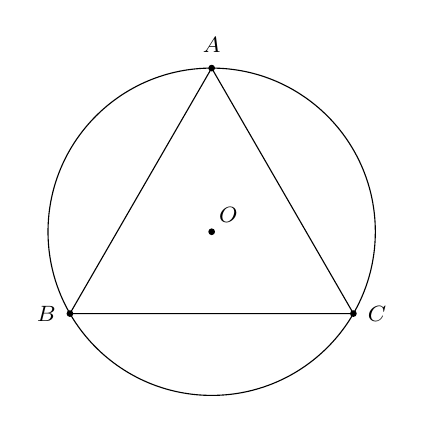
\begin{tikzpicture}[line join=round, line cap=round, >=stealth, font=\footnotesize, scale=1]
				\path
				(0, {1.8*sqrt(3)}) coordinate (A)
				(-1.8,0) coordinate (B)
				(1.8,0) coordinate (C)
				(0, {0.6*sqrt(3)}) coordinate (O);
				
				\draw
				(A)--(B)--(C)--cycle
				(O) circle ({1.2*sqrt(3)});
				
				\foreach \x/\g in {A/90, B/180, C/0, O/45}
				\draw [fill=black](\x) circle (1pt) +(\g:3mm) node {$\x$};
			\end{tikzpicture}
		\end{center}
		\begin{enumerate}
			\item Để vẽ đường tròn ngoại tiếp tam giác $ABC$, ta thực hiện các bước sau
			\begin{itemize}
				\item Vẽ đường trung trực $d_1$ của cạnh $BC$.
				\item Vẽ đường trung trực $d_2$ của cạnh $AC$.
				\item Gọi $O$ là giao điểm của $d_1$ và $d_2$. $O$ chính là tâm đường tròn ngoại tiếp tam giác $ABC$.
				\item Vẽ đường tròn tâm $O$ bán kính $OA$ (hoặc $OB$, hoặc $OC$). Đây là đường tròn ngoại tiếp tam giác $ABC$.
			\end{itemize}
			\textit{Lưu ý:} Do tam giác $ABC$ là tam giác đều, nên tâm $O$ của đường tròn ngoại tiếp cũng chính là trọng tâm, trực tâm và tâm đường tròn nội tiếp của tam giác. Do đó, ta cũng có thể tìm $O$ bằng cách vẽ hai đường trung tuyến (giao điểm là trọng tâm), hoặc hai đường cao (giao điểm là trực tâm), hoặc hai đường phân giác.
			\item Bán kính đường tròn ngoại tiếp $\triangle ABC$ là $R = \dfrac{6\sqrt{3}}{3} = 2\sqrt{3}$ (cm).
		\end{enumerate}
	}
\end{bt}

\begin{bt}%[Dự án EX-9-Đề Cương Toán 9]%[Trần Thanh Phong]%[9H3H1-1]
	Đường tròn ngoại tiếp tam giác đều $ABC$ có bán kính $R = \dfrac{4a\sqrt{3}}{3}$. Tính các cạnh của tam giác $ABC$ theo $a$.
	\begin{center}
		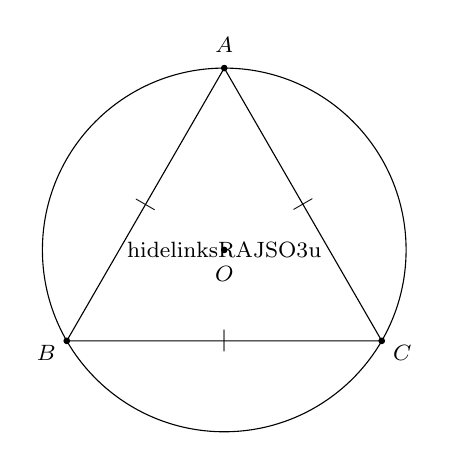
\begin{tikzpicture}[line join=round, line cap=round, >=stealth, font=\footnotesize, scale=1]
			\path
			(0,0) coordinate (O)
			(90:{4*sqrt(3)/3}) coordinate (A)
			(210:{4*sqrt(3)/3}) coordinate (B)
			(-30:{4*sqrt(3)/3}) coordinate (C);
			
			\draw
			(O) circle ({4*sqrt(3)/3})
			(A)--(B) node[midway,sloped]{$|$}
			(B)--(C) node[midway,sloped]{$|$}
			(C)--(A) node[midway,sloped]{$|$}
			% pic[draw, angle radius=3mm, "$60^\circ$", angle eccentricity=2.5] {angle=B--A--C}
			% pic[draw, angle radius=3mm, "$60^\circ$", angle eccentricity=2.5] {angle=C--B--A}
			% pic[draw, angle radius=3mm, "$60^\circ$", angle eccentricity=2.5] {angle=A--C--B}
			;
			
			\foreach \point/\angle in {A/90, B/210, C/-30, O/-90}
			\draw [fill=black] (\point) circle (1pt) +(\angle:3mm) node {$\point$};
			\path (0,0) node{\hypersetup{hidelinks}\href{RAJSO3u}{ }};
		\end{tikzpicture}
	\end{center}
	\loigiai{
		Gọi $x$ là độ dài cạnh của tam giác đều $ABC$ $(x > 0)$.\\
		Khi đó, bán kính của đường tròn ngoại tiếp $\triangle ABC$ là $\dfrac{x\sqrt{3}}{3}$.\\
		Theo đề bài, ta có
		\allowdisplaybreaks
		\begin{eqnarray*} 
			\dfrac{x\sqrt{3}}{3} &=& \dfrac{4a\sqrt{3}}{3} \\
			x &=& 4a.
		\end{eqnarray*}
		Vậy độ dài các cạnh của tam giác đều $ABC$ là $4a$.
	}
\end{bt}

\begin{bt}%[Dự án EX-9-Đề Cương Toán 9]%[Trần Thanh Phong]%[9H3H1-1]
	Cho tam giác $ABC$ đều nội tiếp đường tròn $(O;12\text{ cm})$. Tính độ dài cạnh của tam giác đó.
	\begin{center}
		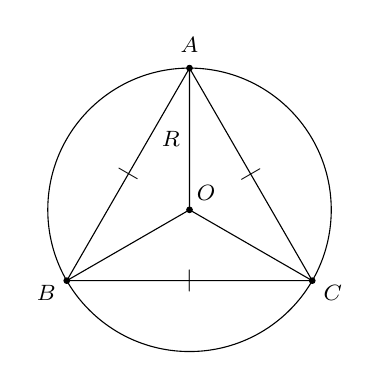
\begin{tikzpicture}[line join=round, line cap=round, >=stealth, font=\footnotesize, scale=1]
			\path
			(0,0) coordinate (O)
			(90:1.8) coordinate (A)
			(210:1.8) coordinate (B)
			(330:1.8) coordinate (C);
			
			\draw
			(O) circle (1.8)
			(O)--(A) node[midway, left]{$R$}
			(O)--(B)
			(O)--(C)
			(A)--(B) node[midway,sloped]{$|$}
			(B)--(C) node[midway,sloped]{$|$}
			(C)--(A) node[midway,sloped]{$|$};
			
			\foreach \x/\g in {O/45, A/90, B/210, C/330}
			\draw [fill=black] (\x) circle (1pt) +(\g:3mm) node {$\x$};
		\end{tikzpicture}
	\end{center}
	\loigiai{
		Gọi $x$ là độ dài cạnh của tam giác đều $ABC$ $(x > 0)$.\\
		Khi đó, bán kính của đường tròn ngoại tiếp tam giác đều $ABC$ là $\dfrac{x\sqrt{3}}{3}$ (cm).\\
		Theo đề bài, ta có
		\begin{eqnarray*}
			\dfrac{x\sqrt{3}}{3} &=& 12\\
			x &=& 12\sqrt{3} \text{ (cm).}
		\end{eqnarray*}
		Vậy độ dài cạnh của tam giác đều $ABC$ là $12\sqrt{3}$ cm.
	}
\end{bt}

\begin{bt}%[Dự án EX-9-Đề Cương Toán 9]%[Trần Thanh Phong]%[9H3V1-1]
	\immini{
		Cho tam giác $DEF$ đều nội tiếp đường tròn $O$ có bán kính bằng $12$ cm. Tính diện tích của tam giác đó.
	}{
		\begin{tikzpicture}[line join=round, line cap=round, >=stealth, font=\footnotesize, scale=1]
			\path
			(0,0) coordinate (O)
			(90:1.8) coordinate (D)
			(210:1.8) coordinate (E)
			(330:1.8) coordinate (F);
			
			\draw
			(O) circle (1.8)
			(O)--(A) node[midway, above, sloped] {$12$ cm}
			(O)--(B)
			(O)--(C)
			(A)--(B) node[midway,sloped]{$|$}
			(B)--(C) node[midway,sloped]{$|$}
			(C)--(A) node[midway,sloped]{$|$};
			
			\foreach \x/\g in {O/45, D/90, E/210, F/330}
			\draw [fill=black] (\x) circle (1pt) +(\g:3mm) node {$\x$};
		\end{tikzpicture}
	}
	\loigiai{
		Gọi $x$ là độ dài cạnh của tam giác đều $DEF$.\\
		Khi đó, bán kính của đường tròn ngoại tiếp tam giác đều $DEF$ là $\dfrac{x\sqrt{3}}{3}$ (cm).\\
		Theo đề bài, ta có
		\begin{eqnarray*}
			\dfrac{x\sqrt{3}}{3} &=& 12\\
			x &=& 12\sqrt{3} \text{ (cm).}
		\end{eqnarray*}
		Diện tích tam giác đều $DEF$ là
		$$ S_{DEF} = \dfrac{\left(12\sqrt{3}\right)^2\sqrt{3}}{4} = 108\sqrt{3} \text{ (cm$^2$).}$$
		Vậy diện tích của tam giác $DEF$ là $108\sqrt{3}$ cm$^2$.
	}
\end{bt}

\begin{bt}%[Dự án EX-9-Đề Cương Toán 9]%[Trần Thanh Phong]%[9H3H1-1]
	\immini{
		Cho tam giác $ABC$ vuông tại $A$ có $AB=10$ cm và $AC=\sqrt{21}$ cm. Tính bán kính đường tròn ngoại tiếp tam giác $ABC$.
	}{
		\begin{tikzpicture}[line join=round, line cap=round, >=stealth, font=\footnotesize, scale=0.7]
			\path
			(-5.5/2,0) coordinate (B)
			(5.5/2,0) coordinate (C)
			({79/22/2}, {10*sqrt(21)/11/2}) coordinate (A)
			($(B)!0.5!(C)$) coordinate (M);
			\draw
			(A)--(B)--(C)--(A)
			(B)--(M) node[midway,sloped]{$|$}
			(M)--(C) node[midway,sloped]{$|$}
			(M) circle (5.5/2)
			pic[draw,angle radius=2.5mm]{right angle = B--A--C};
			\foreach \x/\g in {A/90,B/180,C/0,M/-90}
			\draw [fill=black](\x) circle (1pt) +(\g:3mm) node {$\x$};
		\end{tikzpicture}
	}
	\loigiai{
		Xét $\triangle ABC$ vuông tại $A$, áp dụng định lí Pythagore, ta có
		\allowdisplaybreaks
		\begin{eqnarray*}
			BC^2 &=& AB^2 + AC^2\\
			BC^2 &=& 10^2 + \left(\sqrt{21}\right)^2 \\ 
			BC^2 &=& 121\\
			BC &=& 11 \text{ (cm).}
		\end{eqnarray*}
		Bán kính $R$ của đường tròn ngoại tiếp $\triangle ABC$ là
		$$R = \dfrac{1}{2}BC = \dfrac{1}{2}\cdot 11 = 5{,}5 \text{ (cm).}$$
		Vậy bán kính đường tròn ngoại tiếp tam giác $ABC$ là $5{,}5$ cm.
	}
\end{bt}

\begin{bt}%[Dự án EX-9-Đề Cương Toán 9]%[Trần Thanh Phong]%[9H3H1-1]
	\immini{
		Cho tam giác $DEF$ vuông cân tại $D$ có $DE=15$ cm. Tính bán kính đường tròn ngoại tiếp tam giác $DEF$.
	}{
		\begin{tikzpicture}[line join=round, line cap=round, >=stealth, font=\footnotesize, scale=1]
			\path
			(0,0) coordinate (O)
			($(O) + (0:1.8)$) coordinate (F)
			($(O) + (90:1.8)$) coordinate (D)
			($(O) + (180:1.8)$) coordinate (E)
			;
			\draw
			(D)--(E) node[midway,sloped]{$|$}
			(E)--(F)
			(F)--(D) node[midway,sloped]{$|$}
			(O) circle (1.8)
			pic[draw, angle radius=2.5mm] {right angle = E--D--F};
			\foreach \x/\g in {D/90,E/180,F/0}
			\draw [fill=black](\x) circle (1pt) +(\g:3mm) node {$\x$};
		\end{tikzpicture}
	}
	\loigiai{
		Vì tam giác $DEF$ vuông cân tại $D$ nên ta có $DE = DF = 15$ (cm).\\
		Xét $DEF$ vuông tại $D$, áp dụng định lí Pythagore, ta có
		$$EF = \sqrt{DE^2 + DF^2} = \sqrt{15^2 + 15^2} = 15\sqrt{2} \text{ (cm).}$$
		Bán kính của đường tròn ngoại tiếp tam giác $DEF$ là
		$$R = \dfrac{1}{2}EF = \dfrac{1}{2}\cdot 15\sqrt{2} = \dfrac{15\sqrt{2}}{2} \text{ (cm).}$$
		Vậy bán kính đường tròn ngoại tiếp tam giác $DEF$ là $\dfrac{15\sqrt{2}}{2}$ cm.
	}
\end{bt}

\begin{bt}%[SGK CTST Toán 9]%[Dự án EX-9-Đề Cương Toán 9]%[Trần Thanh Phong]%[9H3H1-1]
	Cho tam giác $ABC$ ($AC < BC$) nội tiếp đường tròn $(O)$ có $AB$ là đường kính. Từ điểm $O$ vẽ đường thẳng song song với $AC$ và cắt đường tròn $(O)$ tại $I$ (điểm $I$ thuộc cung nhỏ $CB$).
	\begin{enumerate}
		\item Chứng minh $OI$ vuông góc với $BC$.
		\item Vẽ tiếp tuyến của đường tròn $(O)$ tại $B$ và cắt đường thẳng $OI$ tại $M$. Chứng minh $MC$ là tiếp tuyến của đường tròn $(O)$.
	\end{enumerate}
	\loigiai{
		\begin{center}
			\begin{tikzpicture}[line join=round, line cap=round, >=stealth, font=\footnotesize, scale=0.7]
				\path
				(0,0) coordinate (O)
				(-3,0) coordinate (A)
				(3,0) coordinate (B)
				({3*cos(120)}, {3*sin(120)}) coordinate (C) 
				({3*cos(60)}, {3*sin(60)}) coordinate (I)   
				(intersection of O--I and C--B) coordinate (K) 
				(3, {3*tan(60)}) coordinate (M)
				;
				\draw
				(O) circle (3)
				(A)--(B)--(M)--(C)--(A) (B)--(C)--(O)--(M)
				;
				\pic[draw,angle radius=2.5mm,angle eccentricity=1.2]{right angle = A--C--B};
				\pic[draw,angle radius=2.5mm,angle eccentricity=1.2]{right angle = O--K--C}; 
				\pic[draw,angle radius=2.5mm,angle eccentricity=1.2]{right angle = O--B--M};
				
				\foreach \p/\g in {O/-90, A/180, B/0, C/135, I/30, M/0, K/10}
				\draw [fill=black](\p) circle (1.2pt) +(\g:4mm) node {$\p$};
			\end{tikzpicture}
		\end{center}
		\begin{enumerate}
			\item Ta có $\widehat{ACB} = 90^\circ$ (góc nội tiếp chắn nửa đường tròn) nên $AC \perp BC$.\\
			Ta có
			\begin{itemize}
				\item $AC\perp BC$ (cmt).
				\item $OI\parallel AC$ (gt).
			\end{itemize}
			Suy ra $OI \perp BC$.
			\item Để chứng minh $MC$ là tiếp tuyến của đường tròn $(O)$, ta cần chứng minh $OC \perp MC$, tức là $\widehat{OCM} = 90^\circ$.\\
			Vì $BM$ là tiếp tuyến của đường tròn $(O)$ tại $B$, nên $OB \perp BM$.
			Do đó, $\widehat{OBM} = 90^\circ$.\\
			Xét $\triangle OBC$ có $OB = OC$ (bán kính của $(O)$) nên $\triangle OBC$ là tam giác cân tại $O$.\\
			Gọi $K$ là giao điểm của $OI$ và $BC$.\\
			Khi đó $OI\perp BC$ tại $K$.\\
			Trong tam giác cân $OBC$, đường thẳng $OK$ là đường cao nên $OK$ cũng là đường phân giác của góc $\widehat{BOC}$.\\
			Suy ra $\widehat{BOK} = \widehat{COK}$ hay $\widehat{BOM} = \widehat{COM}$.\\
			Xét hai tam giác $\triangle OBM$ và $\triangle OCM$, ta có
			\begin{itemize}
				\item $OB = OC$ (cùng là bán kính $R$).
				\item $\widehat{BOM} = \widehat{COM}$ (chứng minh trên).
				\item $OM$ là cạnh chung.
			\end{itemize}
			Suy ra $\triangle OBM = \triangle OCM$ (c.g.c).\\
			Do đó $\widehat{OCM} = \widehat{OBM}$.\\
			Mà $\widehat{OBM} = 90^\circ$ nên $\widehat{OCM} = 90^\circ$.\\
			Vì $C \in (O)$ và $OC \perp MC$ nên $MC$ là tiếp tuyến của đường tròn $(O)$ tại $C$.
		\end{enumerate}
	}
\end{bt}

\subsection{Đường tròn nội tiếp tam giác}
\subsubsection{Kiến thức trọng tâm}
\begin{tomtat}
	\immini{
		\begin{itemize}
			\item Đường tròn tiếp xúc với ba cạnh của tam giác gọi là \textit{đường tròn nội tiếp tam giác}, khi đó tam giác được gọi là \textit{tam giác ngoại tiếp đường tròn}.
			\item Đường tròn nội tiếp tam giác có tâm là giao điểm của ba đường phân giác trong và bán kính bằng khoảng cách từ giao điểm đó đến một cạnh bất kì của tam giác.
		\end{itemize}
	}{
		\begin{tikzpicture}[scale=1, font=\footnotesize,line join=round, line cap=round, >=stealth]
			\draw (0,0) coordinate (B)
			++(60:3) coordinate (A)
			(4,0) coordinate (C)
			($(A)!3cm!(B)$) coordinate (A1)
			($(A)!3cm!(C)$) coordinate (A2)
			($(A1)!.5!(A2)$) coordinate (A3)
			($(B)!3cm!(A)$) coordinate (B1)
			($(B)!3cm!(C)$) coordinate (B2)
			($(B1)!.5!(B2)$) coordinate (B3)
			(intersection of A--A3 and B--B3) coordinate (I)
			($(A)!(I)!(B)$) coordinate (F)
			($(B)!(I)!(C)$) coordinate (D)
			($(A)!(I)!(C)$) coordinate (E)
			;
			\draw (A)--(B)--(C)--cycle (I)--(D) (I)--(E) (I)--(F) (A)--(I)--(B) (I)--(C);
			\draw (I) let\p1=($(I)-(D)$) in circle ({veclen(\x1,\y1)});
			\foreach \i/\g in {A/90,B/180,C/0,D/-90,E/30, F/180,I/-60}{\draw[fill=black](\i) circle (1pt) ($(\i)+(\g:3mm)$) node[scale=1]{$\i$};}
			\draw pic[draw,angle radius=1.5mm]{right angle=C--E--I};
			\draw pic[draw,angle radius=1.5mm]{right angle=A--F--I};
			\draw pic[draw,angle radius=1.5mm]{right angle=B--D--I};
			\draw pic[draw,angle radius=3mm]{angle=F--A--I};
			\draw pic[draw,angle radius=3.8mm]{angle=I--A--E};
			\draw pic[draw,double,angle radius=4mm]{angle=E--C--I};
			\draw pic[draw,double,angle radius=5mm]{angle=I--C--D};
			\draw pic[draw,angle radius=4mm]{angle=D--B--I};
			\draw pic[draw,angle radius=5mm]{angle=I--B--F};
			\draw (.3,.32)--++(45:.2) (.35,.1)--++(20:.2);
		\end{tikzpicture}
	}
\end{tomtat}

\begin{vd}%[SGK CTST Toán 9]%[Dự án EX-9-Đề Cương Toán 9]%[Trần Thanh Phong]%[9H3N1-2]
	Cho góc $xOy$ và đường tròn $(I)$ tiếp xúc với hai cạnh $Ox$, $Oy$. Vẽ tiếp tuyến $d$ của $(I)$ sao cho $d$ cắt $Ox$ tại $A$, cắt $Oy$ tại $B$ và $I$ nằm trong tam giác $OAB$. Tìm đường tròn nội tiếp của tam giác $OAB$.
	\loigiai{
		\immini{
			Ta có đường tròn $(I)$ tiếp xúc với ba cạnh $OA$, $OB$ và $AB$ của tam giác $OAB$ nên $(I)$ là đường tròn nội tiếp tam giác $OAB$.
		}{
			\begin{tikzpicture}[line join=round, line cap=round, >=stealth, font=\footnotesize, scale=1]
				\path
				(0,0) coordinate (O)
				({sqrt(3)}, 1) coordinate (I)
				({2*sqrt(3)}, 0) coordinate (A)
				({sqrt(3)}, 3) coordinate (B)
				({sqrt(3)}, 0) coordinate (P1)
				({sqrt(3)/2}, {3/2}) coordinate (P2)
				({(3*sqrt(3))/2}, {3/2}) coordinate (P3)
				({2*sqrt(3)+0.8}, 0) coordinate (Xrayend)
				({sqrt(3)+0.8*cos(60)}, {3+0.8*sin(60)}) coordinate (Yrayend);
				
				\draw
				(O) -- (Xrayend)
				(O) -- (Yrayend)
				(A) -- (B)
				(I) circle (1)
				(I) -- (P1)
				(I) -- (P2)
				(I) -- (P3)
				pic[draw,angle radius=2.5mm]{right angle = I--P1--A}
				pic[draw,angle radius=2.5mm]{right angle = I--P2--B}
				pic[draw,angle radius=2.5mm]{right angle = I--P3--A};
				
				\node[below=2pt] at (Xrayend) {$x$};
				\node[above=2pt] at (Yrayend) {$y$};
				\node[right=3pt] at (P3) {$d$};
				
				\foreach \x/\g in {O/225, A/-90, B/135, I/-45}
				\draw [fill=black](\x) circle (1pt) +(\g:3mm) node {$\x$};
			\end{tikzpicture}
		}
	}
\end{vd}

\begin{vd}%[SGK CTST Toán 9]%[Dự án EX-9-Đề Cương Toán 9]%[Trần Thanh Phong]%[9H3H1-2]
	Xác định tâm và tính bán kính của đường tròn nội tiếp tam giác đều $ABC$ có độ dài cạnh bằng $a$.
	\loigiai{
		\immini{
			Gọi $O$ là giao điểm của ba đường cao $AH$, $BE$ và $CF$ của tam giác $ABC$.\\
			Ta có tam giác $ABC$ đều nên $AH$, $BE$, $CF$ là ba đường trung tuyến, đồng thời là ba đường phân giác trong của tam giác.\\
			Do đó, $O$ là trọng tâm, đồng thời là tâm đường tròn nội tiếp tam giác $ABC$ với bán kính $r = OH = OE = OF$.\\
			Xét tam giác $\triangle AHB$ vuông tại $H$, ta có 
			$$AH = \sqrt{AB^2 - BH^2} = \sqrt{a^2 - \left(\dfrac{a}{2}\right)^2} = \dfrac{a\sqrt{3}}{2}.$$
			Do đó $r = OH = \dfrac{1}{3}AH = \dfrac{a\sqrt{3}}{6}$.
		}{
			\begin{tikzpicture}[line join=round, line cap=round, >=stealth, font=\footnotesize, scale=1]
				\path
				(-2.25, 0) coordinate (B)
				(2.25, 0) coordinate (C)
				($(B)!0.5!(C)$) coordinate (H)
				(0, {2.25*sqrt(3)}) coordinate (A)
				(0, {0.75*sqrt(3)}) coordinate (O)
				($(A)!0.5!(C)$) coordinate (E)
				($(A)!0.5!(B)$) coordinate (F);
				
				\draw
				(A)--(B)--(C)--cycle
				(A)--(H)
				(B)--(E)
				(C)--(F)
				(O) circle ({0.75*sqrt(3)})
				pic[draw, angle radius=2.5mm]{right angle = C--H--O}
				pic[draw, angle radius=2.5mm]{right angle = A--E--O}
				pic[draw, angle radius=2.5mm]{right angle = B--F--O};
				
				\foreach \point/\pos in {A/90, B/210, C/-30, H/-90, O/60, E/30, F/150}
				\draw [fill=black] (\point) circle (1pt) +(\pos:3mm) node {$\point$};
			\end{tikzpicture}
		}
	}
\end{vd}

\begin{luuy}
	\begin{itemize}
		\item Đường tròn nội tiếp tam giác đều cạnh $a$ có tâm là trọng tâm của tam giác và bán kính bằng $\dfrac{a\sqrt{3}}{6}$.
		\item Tam giác đều có tâm đường tròn nội tiếp và tâm đường tròn ngoại tiếp trùng nhau.
	\end{itemize}
\end{luuy}

\subsubsection{Bài tập}

\begin{bt}%[SGK CTST Toán 9]%[Dự án EX-9-Đề Cương Toán 9]%[Trần Thanh Phong]%[9H3N1-2]
	Cho tam giác đều $ABC$ có cạnh bằng $6$ cm.
	\begin{enumerate}
		\item Nêu cách vẽ đường tròn nội tiếp tam giác $ABC$.
		\item Tính bán kính $r$ của đường tròn nội tiếp tam giác $ABC$.
	\end{enumerate}
	\loigiai{
		\begin{center}
			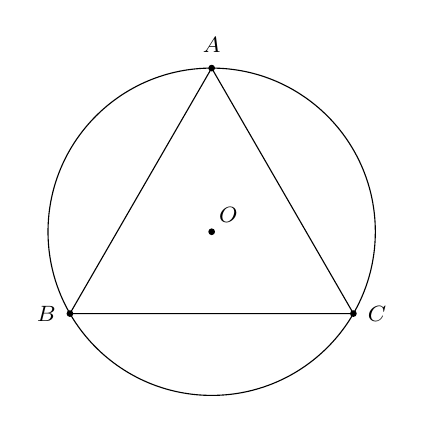
\begin{tikzpicture}[line join=round, line cap=round, >=stealth, font=\footnotesize, scale=1]
				\path
				(0, {1.8*sqrt(3)}) coordinate (A)
				(-1.8,0) coordinate (B)
				(1.8,0) coordinate (C)
				(0, {0.6*sqrt(3)}) coordinate (O);
				
				\draw
				(A)--(B)--(C)--cycle
				(O) circle ({1.2*sqrt(3)});
				
				\foreach \x/\g in {A/90, B/180, C/0, O/45}
				\draw [fill=black](\x) circle (1pt) +(\g:3mm) node {$\x$};
			\end{tikzpicture}
		\end{center}
		\begin{enumerate}
			\item Để vẽ đường tròn nội tiếp tam giác $ABC$, ta thực hiện các bước sau
			\begin{itemize}
				\item Vẽ đường phân giác của một góc bất kỳ của tam giác, ví dụ góc $A$. Gọi đường phân giác này là $d_1$.
				\item Vẽ đường phân giác của một góc khác, ví dụ góc $B$. Gọi đường phân giác này là $d_2$.
				\item Gọi $O$ là giao điểm của hai đường phân giác $d_1$ và $d_2$. Điểm $O$ này chính là tâm của đường tròn nội tiếp tam giác $ABC$.
				\item Từ tâm $O$, kẻ một đường thẳng vuông góc với một cạnh bất kỳ của tam giác. Ví dụ, kẻ $OM \perp BC$ (trong đó $M$ là chân đường vuông góc trên cạnh $BC$). Độ dài đoạn thẳng $OM$ chính là bán kính $r$ của đường tròn nội tiếp.
				\item Vẽ đường tròn tâm $O$ với bán kính $r = OM$. Đường tròn này là đường tròn nội tiếp tam giác $ABC$.
			\end{itemize}
			\textit{Lưu ý:} Do tam giác $ABC$ là tam giác đều, các đường phân giác cũng đồng thời là các đường trung tuyến, đường cao, và đường trung trực của tam giác. Do đó, tâm $O$ của đường tròn nội tiếp cũng chính là trọng tâm, trực tâm, và tâm đường tròn ngoại tiếp của tam giác. Một cách đơn giản để xác định $O$ trong trường hợp tam giác đều là vẽ hai đường trung tuyến, giao điểm của chúng chính là $O$.
			\item Bán kính của đường tròn nội tiếp $\triangle ABC$ là
			$r = \dfrac{6\sqrt{3}}{6} = \sqrt{3}$ (cm).
		\end{enumerate}
	}
\end{bt}

\begin{bt}%[Dự án EX-9-Đề Cương Toán 9]%[Trần Thanh Phong]%[9H3H1-2]
	Cho tam giác $DEF$ đều ngoại tiếp đường tròn $(O;3 \text{ cm})$. Tính độ dài cạnh của tam giác đó.
	\begin{center}
		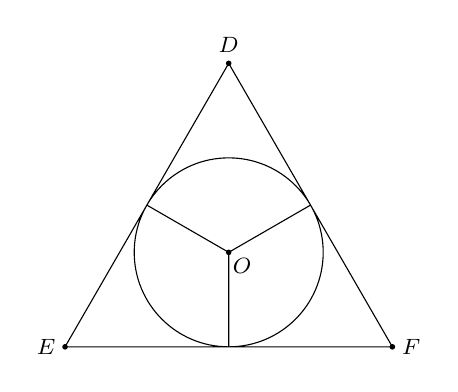
\begin{tikzpicture}[line join=round, line cap=round, >=stealth, font=\footnotesize, scale=0.8]
			\path
			(0,0) coordinate (O)
			(0,{2*1.5}) coordinate (D)
			({-1.5*sqrt(3)}, {-1.5}) coordinate (E)
			({1.5*sqrt(3)}, {-1.5}) coordinate (F)
			(0,{-1.5}) coordinate (P1)
			({0.75*sqrt(3)}, {0.75}) coordinate (P2)
			({-0.75*sqrt(3)}, {0.75}) coordinate (P3);
			
			\draw
			(O) circle (1.5)
			(D)--(E)
			(E)--(F)
			(F)--(D)
			(O)--(P1)
			(O)--(P2)
			(O)--(P3);
			
			\foreach \centerpoint/\firstpoint/\secondpoint in {P1/O/E, P2/O/F, P3/O/D}
			pic[draw, angle radius=3mm]{right angle = \firstpoint--\centerpoint--\secondpoint};
			
			\foreach \point/\angle in {O/-45, D/90, E/180, F/0}
			\draw [fill=black] (\point) circle (1pt) +(\angle:3mm) node {$\point$};
		\end{tikzpicture}
	\end{center}
	\loigiai{
		Gọi $x$ (cm) là độ dài cạnh của tam giác đều $DEF$ $(x > 0)$.\\
		Bán kính của đường tròn nội tiếp $\triangle DEF$ là
		$\dfrac{x\sqrt{3}}{6}$ (cm$^3$).\\
		Theo đề bài, ta có
		\begin{eqnarray*}
			\dfrac{x\sqrt{3}}{6} &=& 3\\
			x &=& 6\sqrt{3} \text{ (cm).}
		\end{eqnarray*}
		Vậy độ dài cạnh của tam giác đều $DEF$ là $6\sqrt{3}$ cm.
	}
\end{bt}

\begin{bt}%[SGK CTST Toán 9]%[Dự án EX-9-Đề Cương Toán 9]%[9H3H1-2]
	Tính diện tích tam giác đều có bán kính đường tròn nội tiếp bằng $1$ cm.
	\loigiai{
		Tam giác đều có bán kính đường tròn nội tiếp bằng $1$ cm thì có cạnh bằng 
		$$1 : \dfrac{\sqrt{3}}{6}=2\sqrt{3} \text{ (cm).}$$
		Diện tích tam giác đều đó là
		$$S = \dfrac{\left(2\sqrt{3}\right)^2\sqrt{3}}{4} = 3\sqrt{3} \text{ (cm$^2$).}$$
	}
\end{bt}

\begin{bt}%[Dự án EX-9-Đề Cương Toán 9]%[Trần Thanh Phong]%[9H3H1-2]
	Cho tam giác $MNP$ đều có cạnh bằng $10$ cm. Tính bán kính đường tròn ngoại tiếp và bán kính đường tròn nội tiếp của tam giác đó.
	\begin{center}
		\begin{tikzpicture}[line join=round, line cap=round, >=stealth, font=\footnotesize, scale=0.6]
			\path
			(0,0) coordinate (N)
			({10 * 2/3},0) coordinate (P)
			({5 * 2/3}, {5*sqrt(3) * 2/3}) coordinate (M)
			({5 * 2/3}, {5*sqrt(3)/3 * 2/3}) coordinate (O)
			($(N)!0.5!(P)$) coordinate (NP_mid);
			\draw
			(M)--(N)--(P)--cycle
			(O) circle ({10*sqrt(3)/3 * 2/3})
			(O) circle ({5*sqrt(3)/3 * 2/3});
			\foreach \x/\g/\lbl in {M/90/$M$, N/210/$N$, P/330/$P$, O/0/$O$}
			\draw [fill=black] (\x) circle (1pt) +(\g:4mm) node {\lbl};
			\node[below=3pt] at (NP_mid) {$10$};
		\end{tikzpicture}
	\end{center}
	\loigiai{
		Bán kính của đường tròn ngoại tiếp $\triangle MNP$ là
		$$R = \dfrac{10\sqrt{3}}{3} \text{ (cm).}$$
		Bán kính của đường tròn nội tiếp $\triangle MNP$ là
		$$r = \dfrac{10\sqrt{3}}{6} = \dfrac{5\sqrt{3}}{3} \text{ (cm).}$$
	}
\end{bt}

\begin{bt}%[Dự án EX-9-Đề Cương Toán 9]%[Trần Thanh Phong]%[9H3V1-2]
	\immini{
		Đường tròn ngoại tiếp tam giác đều $ABC$ có bán kính $R = \dfrac{4a\sqrt{3}}{3}$. Tính bán đường tròn nội tiếp tam giác $ABC$ theo $a$.
	}{
		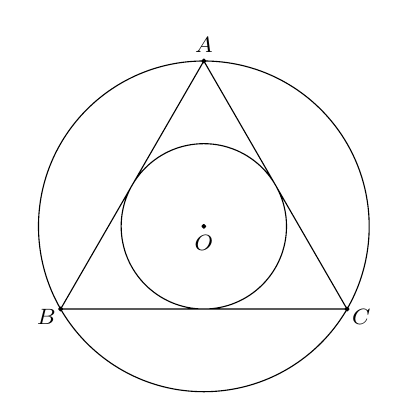
\begin{tikzpicture}[line join=round, line cap=round, >=stealth, font=\footnotesize, scale=0.7]
			\path
			(0,0) coordinate (O)
			({0},{3}) coordinate (A)
			({3*cos(210)}, {3*sin(210)}) coordinate (B)
			({3*cos(330)}, {3*sin(330)}) coordinate (C);
			\draw
			(O) circle (3)
			(O) circle (1.5)
			(A)--(B)--(C)--(A);
			\foreach \x/\g in {A/90, B/210, C/330, O/-90}
			\draw [fill=black](\x) circle (1pt) +(\g:3mm) node {$\x$};
		\end{tikzpicture}
	}
	\loigiai{
		\immini{
			Ta có $O$ vừa là tâm đường tròn nội tiếp vừa là tâm đường tròn ngoại tiếp của $\triangle ABC$.\\
			Vì $\triangle ABC$ đều nên $AH$, $BE$, $CF$ vừa là ba đường phân giác, đồng thời là ba đường trung tuyến.\\
			Suy ra $AO = 2OH$ hay $R = 2r$ do đó
			$$r = \dfrac{1}{2}R = \dfrac{1}{2} \cdot \dfrac{4a\sqrt{3}}{3} = \dfrac{2a\sqrt{3}}{3}.$$
			Vậy bán kính đường tròn nội tiếp tam giác $ABC$ là $\dfrac{2a\sqrt{3}}{3}$.
		}{
			\begin{tikzpicture}[line join=round, line cap=round, >=stealth, font=\footnotesize, scale=1]
				\path
				(-2.25, 0) coordinate (B)
				(2.25, 0) coordinate (C)
				($(B)!0.5!(C)$) coordinate (H)
				(0, {2.25*sqrt(3)}) coordinate (A)
				(0, {0.75*sqrt(3)}) coordinate (O)
				($(A)!0.5!(C)$) coordinate (E)
				($(A)!0.5!(B)$) coordinate (F);
				
				\draw
				(A)--(B)--(C)--cycle
				(A)--(H)
				(B)--(E)
				(C)--(F)
				(O) circle ({0.75*sqrt(3)})
				(O) circle (2.6)
				pic[draw, angle radius=2.5mm]{right angle = C--H--O}
				pic[draw, angle radius=2.5mm]{right angle = A--E--O}
				pic[draw, angle radius=2.5mm]{right angle = B--F--O};
				
				\foreach \point/\pos in {A/90, B/210, C/-30, H/-90, O/60, E/30, F/150}
				\draw [fill=black] (\point) circle (1pt) +(\pos:3mm) node {$\point$};
			\end{tikzpicture}
		}
	}
\end{bt}

\begin{bt}%[SGK CTST Toán 9]%[Dự án EX-9-Đề Cương Toán 9]%[Trần Thanh Phong]%[9H3V1-2]
	\immini{
		Cho tam giác $ABC$ ngoại tiếp đường tròn $(I)$. Gọi $D$, $E$, $F$ lần lượt là các tiếp điểm của đường tròn $(I)$ với các cạnh $AB$, $BC$, $AC$.
		\begin{enumerate}
			\item Chứng minh $2AD = AB + AC - BC$.
			\item Tìm các hệ thức tương tự như hệ thức ở câu trên.
		\end{enumerate}
	}{
		\begin{tikzpicture}[line join=round, line cap=round, >=stealth, font=\footnotesize, scale=0.8]
			\path
			(0,0) coordinate (B)
			(6.5,0) coordinate (C) 
			(1.5,4) coordinate (A)
			({(6.5*1.5 + sqrt(pow(6.5-1.5,2)+pow(0-4,2))*0 + sqrt(pow(1.5-0,2)+pow(4-0,2))*6.5)/(6.5 + sqrt(pow(6.5-1.5,2)+pow(0-4,2)) + sqrt(pow(1.5-0,2)+pow(4-0,2)) )}, {(6.5*4 + sqrt(pow(6.5-1.5,2)+pow(0-4,2))*0 + sqrt(pow(1.5-0,2)+pow(4-0,2))*0)/(6.5 + sqrt(pow(6.5-1.5,2)+pow(0-4,2)) + sqrt(pow(1.5-0,2)+pow(4-0,2)) )}) coordinate (I)
			($(A)!(I)!(B)$) coordinate (D)
			($(B)!(I)!(C)$) coordinate (E)
			($(A)!(I)!(C)$) coordinate (F);
			
			\draw
			(A)--(B)--(C)--cycle
			(I) circle ({0.5*6.5*4 / (0.5*(6.5 + sqrt(pow(6.5-1.5,2)+pow(0-4,2)) + sqrt(pow(1.5-0,2)+pow(4-0,2))))})
			(I)--(D)
			(I)--(E)
			(I)--(F)
			pic[draw,angle radius=2mm]{right angle = A--D--I}
			pic[draw,angle radius=2mm]{right angle = B--E--I}
			pic[draw,angle radius=2mm]{right angle = A--F--I};
			
			\foreach \p/\g in {A/90, B/180, C/0, I/-10, D/170, E/-90, F/45}
			\draw [fill=black] (\p) circle (1pt) +(\g:3.4mm) node {$\p$};
		\end{tikzpicture}
	}
	\loigiai{
		\begin{enumerate}
			\item Vì đường tròn $(I)$ tiếp xúc với các cạnh $AB$, $BC$, $AC$ lần lượt tại $D$, $E$, $F$, theo tính chất hai tiếp tuyến cắt nhau, ta có $AD = AF$, $BD = BE$, $CE = CF$.
			\allowdisplaybreaks
			\begin{eqnarray*}
				AB+AC-BC &=& (AD+DB) + (AF+FC) - (BE+EC) \\
				&=& (AD+BE) + (AD+CE) - (BE+CE) \\
				&=& AD+BE+AD+CE-BE-CE \\
				&=& 2AD + (BE-BE) + (CE-CE) \\
				&=& 2AD.
			\end{eqnarray*}
			Vậy $2AD = AB+AC-BC$.
			\item Các hệ thức tương tự như hệ thức ở câu trên là
			\begin{itemize}
				\item $2BD = AB+BC-AC$.
				\item $2CE = AC+BC-AB$.
			\end{itemize}
			Vì $AD=AF$, $BD=BE$, $CE=CF$, các hệ thức trên cũng có thể viết cho $AF$, $BE$, $CF$ như sau
			\begin{itemize}
				\item $2AF = AB+AC-BC$.
				\item $2BE = AB+BC-AC$.
				\item $2CF = AC+BC-AB$.
			\end{itemize}
		\end{enumerate}
	}
\end{bt}

\begin{bt}%[Dự án EX-9-Đề Cương Toán 9]%[Trần Thanh Phong]%[9H3N1-3]
	\immini{
		Một công ty muốn thiết kế một biển báo hình tam giác đều có cạnh $21\sqrt{3}$ cm để đặt vừa khít một logo hình tròn bên trong (như hình vẽ). Tính bán kính của logo hình tròn đó.
	}{
		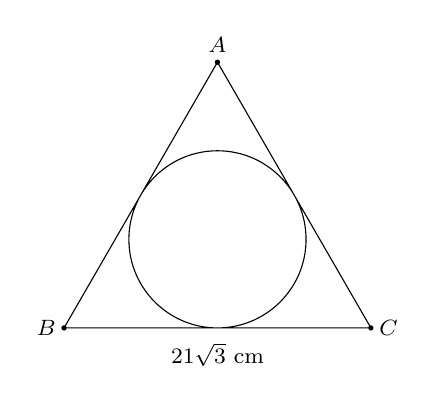
\begin{tikzpicture}[line join=round, line cap=round, >=stealth, font=\footnotesize, scale=0.75]
			\path
			(0, {1.5}) coordinate (O)
			(0, {3*1.5}) coordinate (A)
			({-1.5*sqrt(3)}, 0) coordinate (B)
			({1.5*sqrt(3)}, 0) coordinate (C);
			\draw
			(A)--(B)
			(C)--(A)
			(B)--(C) node[midway, below=2pt] {$21\sqrt{3}$ cm}
			(O) circle ({1.5});
			\foreach \x/\g in {A/90, B/180, C/0}
			\draw [fill=black](\x) circle (1pt) +(\g:3mm) node {$\x$};
		\end{tikzpicture}
	}
	\loigiai{
		Bán kính của logo hình tròn đó là
		$$ r = \dfrac{21\sqrt{3}\cdot\sqrt{3}}{6} 
		= \dfrac{21}{2} \text{ (cm).}$$
	}
\end{bt}

\begin{bt}%[Dự án EX-9-Đề Cương Toán 9]%[Trần Thanh Phong]%[9H3H1-3]
	\immini{
		Người ta muốn làm một khung gỗ hình tam giác đều có cạnh $10\sqrt{10}$ cm để đặt vừa khít một đồng hồ treo tường (như hình vẽ). Tính đường kính chiếc đồng hồ đó.
	}{
		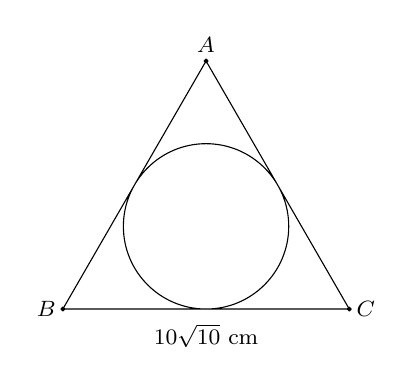
\begin{tikzpicture}[line join=round, line cap=round, >=stealth, font=\footnotesize, scale=0.7]
			\path
			(0, {1.5}) coordinate (O)
			(0, {3*1.5}) coordinate (A)
			({-1.5*sqrt(3)}, 0) coordinate (B)
			({1.5*sqrt(3)}, 0) coordinate (C);
			\draw
			(A)--(B)
			(C)--(A)
			(B)--(C) node[midway, below=2pt] {$10\sqrt{10}$ cm}
			(O) circle ({1.5});
			\foreach \x/\g in {A/90, B/180, C/0}
			\draw [fill=black](\x) circle (1pt) +(\g:3mm) node {$\x$};
		\end{tikzpicture}
	}
	\loigiai{
		Ta thấy chiếc đồng hồ có dạng hình tròn nội tiếp $\triangle ABC$.\\
		Bán kính của đường tròn nội tiếp $\triangle ABC$ là
		$$ r = \dfrac{10\sqrt{10} \cdot \sqrt{3}}{6} 
		= \dfrac{5\sqrt{30}}{3} \text{ (cm).}$$
		Đường kính của chiếc đồng hồ là
		$$ d = 2r = 2\cdot\dfrac{5\sqrt{30}}{3} = \dfrac{10\sqrt{30}}{3} \text{ (cm).}$$
		Vậy đường kính chiếc đồng hồ đó là $\dfrac{10\sqrt{30}}{3}$ cm.
	}
\end{bt}

\begin{bt}%[Dự án EX-9-Đề Cương Toán 9]%[Trần Thanh Phong]%[9H3C1-3]
	Bác An có một khu đất được bao xung quanh bởi ba con đường thẳng lập thành một tam giác với độ dài các cạnh là $AB = 30$ m, $AC = 40$ m, $BC = 50$ m (như hình vẽ).
	\immini{
		\begin{enumerate}
			\item Với giá đất hiện tại là $20$ triệu/m$^2$. Nếu Bác An bán thì được bao nhiêu tiền?
			\item Bác An muốn xây một ngôi nhà biệt thự bên trong khu đất mình cách đều cả ba con đường đó. Khi đó, ngôi nhà biệt thự của Bác An cách mỗi con đường là bao nhiêu?
		\end{enumerate}
	}{
		\begin{tikzpicture}[line join=round, line cap=round, >=stealth, font=\footnotesize, scale=1]
			\path
			(0,0) coordinate (B)
			(5,0) coordinate (C)
			(1.8,2.4) coordinate (A)
			(2,1) coordinate (I)
			($(A)!(I)!(B)$) coordinate (D) 
			($(B)!(I)!(C)$) coordinate (E)
			($(A)!(I)!(C)$) coordinate (F);
			
			\draw
			(A)--(B) node[midway, sloped, above=1pt] {$30$ m}
			(B)--(C) node[midway, below=2pt] {$50$ m}
			(C)--(A) node[midway, sloped, above=1pt] {$40$ m}
			(I)--(D)
			(I)--(E)
			(I)--(F)
			(I) circle (1);
			
			\foreach \p/\g in {A/90, B/180, C/0, I/-45}
			\draw [fill=black] (\p) circle (1pt) +(\g:3mm) node {$\p$};
			
			\foreach \ptA/\ptB/\ptC in {B/A/C, B/D/I, B/E/I, C/F/I}
			\pic[draw,angle radius=2.5mm]{right angle = \ptA--\ptB--\ptC};
		\end{tikzpicture}
	}
	\loigiai{
		\begin{center}
			\begin{tikzpicture}[line join=round, line cap=round, >=stealth, font=\footnotesize, scale=1]
				\path
				(0,0) coordinate (B)
				(5,0) coordinate (C)
				(1.8,2.4) coordinate (A)
				(2,1) coordinate (I)
				($(A)!(I)!(B)$) coordinate (D) 
				($(B)!(I)!(C)$) coordinate (E)
				($(A)!(I)!(C)$) coordinate (F);
				
				\draw
				(A)--(B)--(C)--(A)
				(E)--(I)--(E)
				(D)--(I)--(F) 
				(I) circle (1);
				
				\foreach \p/\g in {A/90, B/180, C/0, I/-45,D/135,E/-90,F/45}
				\draw [fill=black] (\p) circle (1pt) +(\g:3mm) node {$\p$};
				
				\foreach \ptA/\ptB/\ptC in {B/A/C, B/D/I, B/E/I, C/F/I}
				\pic[draw,angle radius=2.5mm]{right angle = \ptA--\ptB--\ptC};
			\end{tikzpicture}
		\end{center}
		\begin{enumerate}
			\item Xét $\triangle ABC$, ta có
			\begin{itemize}
				\item $AB^2 + AC^2 = 30^2 + 40^2 = 900 + 1600 = 2500$.
				\item $BC^2 = 50^2 = 2500$.
			\end{itemize}
			Suy ra $AB^2 + AC^2 = BC^2$ nên tam giác $ABC$ vuông tại $A$ theo định lí Pythagore đảo.\\
			Diện tích khu đất hình tam giác $ABC$ là
			$$S_{ABC} = \dfrac{1}{2}\cdot AB\cdot AC = \dfrac{1}{2}\cdot 30\cdot 40 = 600 \text{ (m$^2$).}$$ 
			Số tiền Bác An thu được nếu bán khu đất trên là
			$600\cdot 20 = 12\,000$ (triệu đồng).\\
			Vậy nếu Bác An bán khu đất thì được $12\,000$ triệu đồng.
			\item
			Bác An muốn xây một ngôi nhà biệt thự bên trong khu đất cách đều cả ba con đường (tức là cách đều ba cạnh của tam giác $ABC$).\\
			Khi đó, vị trí ngôi nhà là tâm $I$ của đường tròn nội tiếp tam giác $ABC$.
			Khoảng cách từ ngôi nhà đến mỗi con đường chính là bán kính $r$ của đường tròn nội tiếp tam giác $ABC$.\\
			Xét $(I)$, ta có $AB$, $AC$, $BC$ là các tiếp tiếp của $(I)$.\\
			Gọi $D$, $E$, $F$ lần lượt là tiếp điểm của các tiếp tuyến $AB$, $AC$, $BC$ với $(I)$.\\
			Theo tính chất hai tiếp tuyến cắt nhau, ta có $AD=AF$, $BD=BE$, $CE=CF$.
			\allowdisplaybreaks
			\begin{eqnarray*}
				AB+AC-BC &=& (AD+DB) + (AF+FC) - (BE+EC) \\
				&=& (AD+BE) + (AD+CE) - (BE+CE) \\
				&=& AD+BE+AD+CE-BE-CE \\
				&=& 2AD + (BE-BE) + (CE-CE) \\
				&=& 2AD.
			\end{eqnarray*}
			Vậy $2AD = AB+AC-BC$ hay $AD = \dfrac{AB+AC-BC}{2}$. $\quad (1)$\\
			Xét tứ giác $ADIF$ có $\widehat{DAF}=\widehat{ADI}=\widehat{AFI}=90^\circ$ do đó tứ giác $ADIF$ là hình chữ nhật nên $AD = ID$. $\quad (2)$\\
			Từ $(1)$ và $(2)$, suy ra 
			$$ID = \dfrac{AB+AC-BC}{2} = \dfrac{30+40-50}{2} = 10 \text{ (m).}$$
			Vậy ngôi nhà biệt thự của Bác An cách mỗi con đường là $10$ m.
		\end{enumerate}
	}
\end{bt}

